\documentclass[journal]{IEEEtran}
%------------------------------------------------------------------------------
% Online Supplementary Material for the TGRS submission (tgrs-article.tex).
% Holds non-essential content relocated from the main paper. Floats are
% numbered S1, S2, ... and referenced from the main text as Sec./Table/Fig. S#.
%------------------------------------------------------------------------------
\usepackage{amsmath,amssymb,amsfonts}
\usepackage{graphicx}
\graphicspath{{figures/}}
\usepackage{booktabs}
\usepackage{array}
\usepackage{xcolor}
\usepackage{url}
\usepackage[hidelinks]{hyperref}

% S-prefixed float and equation numbering
\renewcommand{\thefigure}{S\arabic{figure}}
\renewcommand{\thetable}{S\arabic{table}}
\renewcommand{\theequation}{S\arabic{equation}}
\renewcommand{\thesection}{S-\Alph{section}}

\begin{document}

\title{Supplementary Material:\\Deep Architectures Can Generalize: Sparse Feature Selection Improves Spatial Transfer in Earth Observation}
\author{Michael~L.~Mann, Sairam~Venkatachalam, Disha~Kacha, Devarsh~Sheth, Ryan~Engstrom, and Amir~Jafari}
\markboth{IEEE Transactions on Geoscience and Remote Sensing --- Supplementary Material}{}
\maketitle

\noindent This document collects supporting material for the main paper. Section~S-A details the
dataset, feature set, and model definitions; Section~S-B defines the metrics; Section~S-C reports
training cost; Section~S-D presents the ablation studies; Section~S-E the data-efficiency experiment;
and Section~S-F the raw-versus-\texttt{xr\_fresh} representation comparison. Equation, figure, table,
and section labels are prefixed ``S''.

\section{Dataset Details, Feature Set, and Model Definitions}
\label{sec:models}
\emph{Supports main paper Sec.~II--III.}

\subsection{Exploratory Data Analysis}
The five crop classes are heavily imbalanced (Fig.~\ref{sfig:fields}). Lucerne/medics dominates
both regions despite having the smallest mean field area (Fig.~\ref{sfig:area}). Spectral responses
overlap substantially across crops (Fig.~\ref{sfig:box}), and wheat and barley are especially
similar (Fig.~\ref{sfig:wb}), which is the dominant source of persistent confusion noted in the main
paper.

\begin{figure}[!t]
\centering

\includegraphics[width=\columnwidth]{fields_count.pdf}
\caption{Number of fields per crop type in the training and holdout regions.}
\label{sfig:fields}
\end{figure}

\begin{figure}[!t]
\centering

\includegraphics[width=\columnwidth]{avg_field_area.pdf}
\caption{Average field area by crop type (hectares).}
\label{sfig:area}
\end{figure}

\begin{figure}[!t]
\centering

\includegraphics[width=\columnwidth]{all_crops_boxplot.pdf}
\caption{Spectral band intensities by crop type. The substantial overlap shows that classification
from a limited set of spectral bands alone is challenging.}
\label{sfig:box}
\end{figure}

\begin{figure}[!t]
\centering

\includegraphics[width=\columnwidth]{wheat_barley_boxplot.pdf}
\caption{Wheat versus barley spectral band intensities. The high similarity motivates their
persistent classification confusion across all models.}
\label{sfig:wb}
\end{figure}

\subsection{\texttt{xr\_fresh} Feature Set}
Table~\ref{stab:features} lists the time-series features extracted from each pixel's 10-month
spectral profile with \texttt{xr\_fresh} \cite{mann2023, mann2025}, forming the 174-dimensional
per-pixel vector used by the classical learners (Fig.~\ref{sfig:tsfeat} illustrates the extraction).

\begin{table}[!t]
\centering
\footnotesize
\caption{Time-series features extracted from each pixel's spectral profile with \texttt{xr\_fresh}.}
\label{stab:features}
\renewcommand{\arraystretch}{1.15}
\begin{tabular}{@{}>{\raggedright\arraybackslash}p{0.32\columnwidth}p{0.60\columnwidth}@{}}
\toprule
\textbf{Feature} & \textbf{Description} \\
\midrule
Absolute Energy & Sum of squared values. \\
Absolute Sum of Changes & Total absolute difference between consecutive measurements. \\
Autocorrelation (1, 2-month lag) & Correlation with one- and two-month lagged versions. \\
Count Above Mean & Number of points above the series mean. \\
Day of Year of Max/Min & Julian day of the maximum and minimum. \\
Kurtosis & Tail heaviness of the distribution. \\
Linear Trend & Slope of a least-squares fit. \\
Longest Strike Above/Below Mean & Longest consecutive run above or below the mean. \\
Max/Min & Absolute extreme values. \\
Mean/Median & Measures of central tendency. \\
Mean Absolute Change/Mean Change & Average magnitude and signed change between points. \\
Mean Second Derivative & Mean of the series' second differences. \\
Quantiles (0.05, 0.95) & 5th and 95th percentiles. \\
Ratio Beyond $r\sigma$ & Proportion of points more than $r$ s.d.\ ($r=1,2,3$) from the mean. \\
Skewness & Asymmetry around the mean. \\
Standard Deviation/Variance & Spread measures. \\
Sum of Values & Total sum of observations. \\
Symmetry Looking & Similarity under series reversal. \\
Time Series Complexity & Complexity-Invariant Distance metric of irregularity. \\
\bottomrule
\end{tabular}
\end{table}

\begin{figure}[!t]
\centering
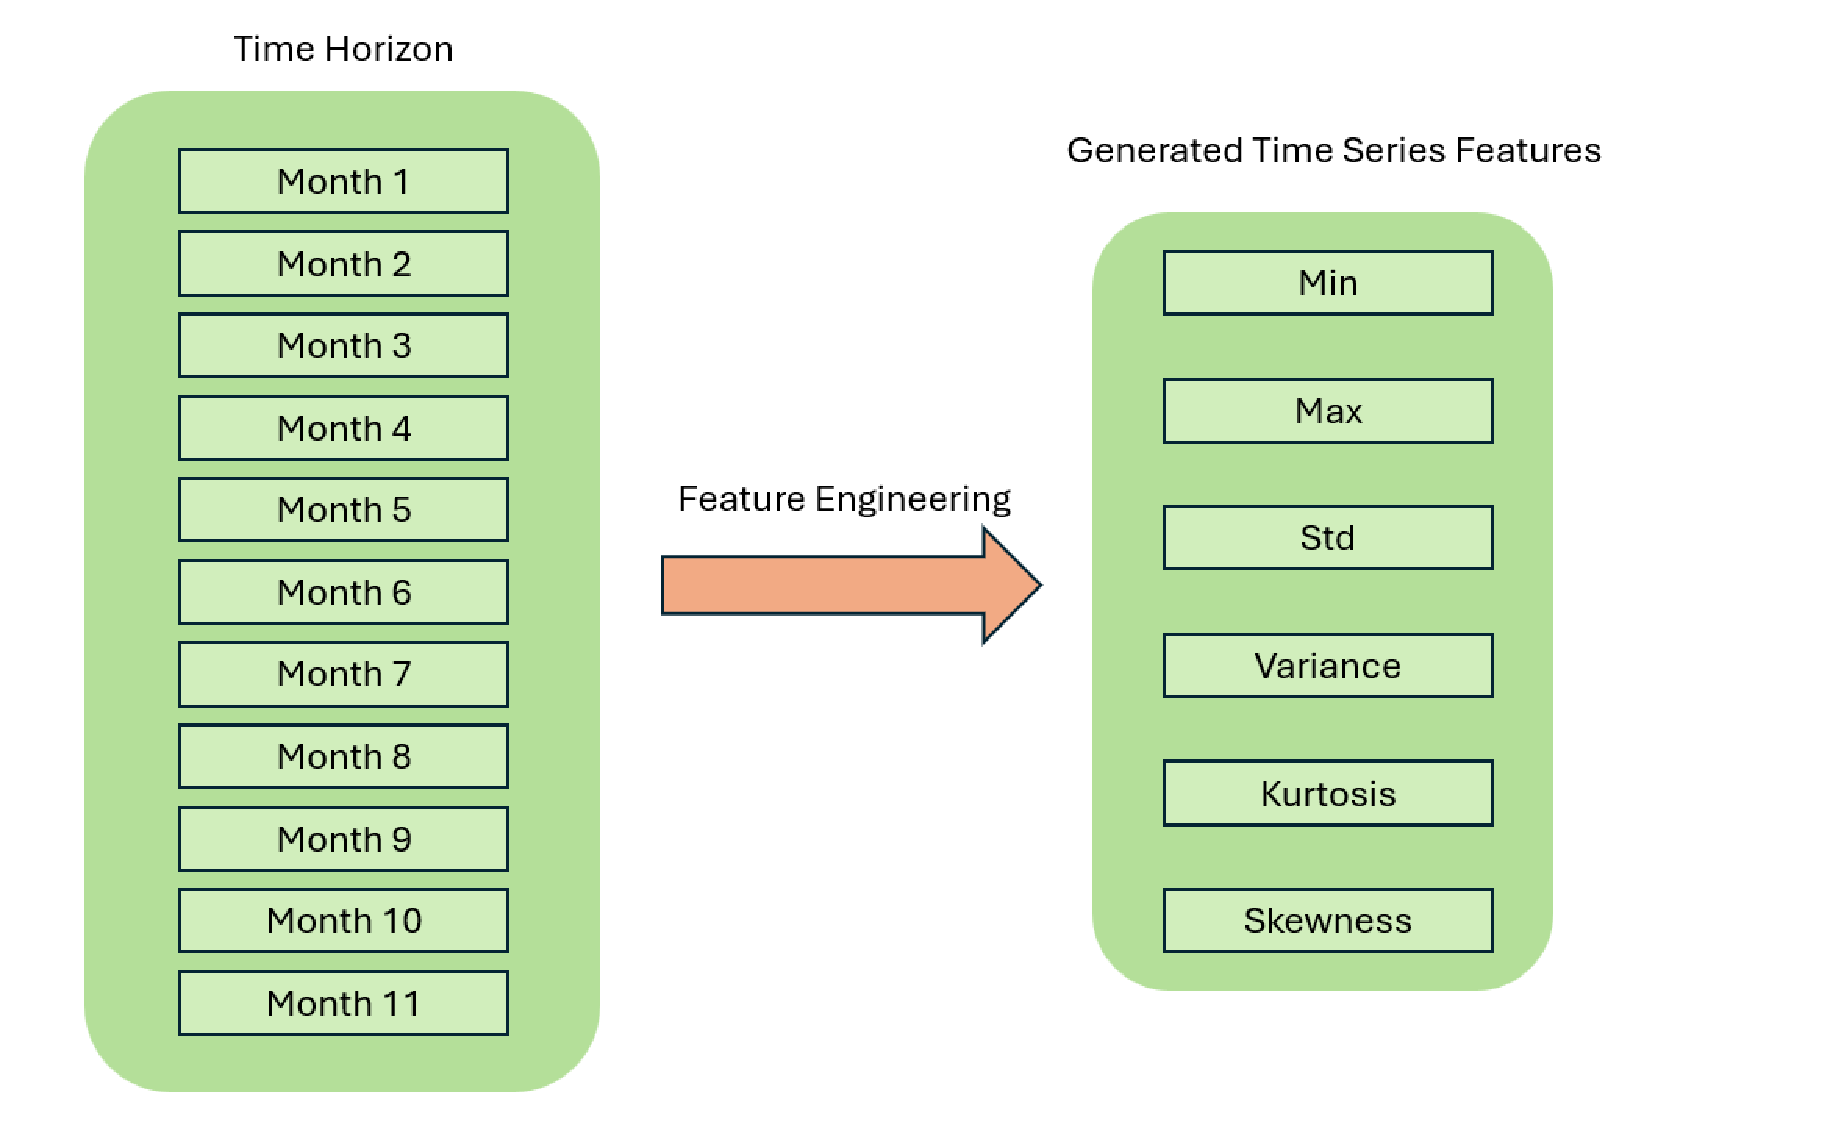
\includegraphics[width=\columnwidth]{Time_Series_Feature_Generation.pdf}
\caption{Extraction of statistical and temporal features from the 10-month spectral time series.}
\label{sfig:tsfeat}
\end{figure}

\subsection{Baseline Classical Model Definitions}
For a feature vector $\mathbf{x}_i$ and class $c\in\{1,\dots,C\}$, the four baselines are as follows.
Logistic regression \cite{james2013} (multinomial):
\begin{equation}
P(y_i = c \mid \mathbf{x}_i) =
\frac{\exp(\mathbf{w}_c^\top \mathbf{x}_i + b_c)}{\sum_{c'=1}^{C} \exp(\mathbf{w}_{c'}^\top \mathbf{x}_i + b_{c'})}.
\end{equation}
Random Forest \cite{breiman2001}: majority vote over $K$ trees,
$\hat{y}_i = \operatorname{mode}\{T_1(\mathbf{x}_i),\dots,T_K(\mathbf{x}_i)\}$.
LightGBM \cite{ke2017}: additive boosting with rate $\eta$,
$\hat{y}_i^{(t)} = \hat{y}_i^{(t-1)} + \eta\, f_t(\mathbf{x}_i)$.
XGBoost \cite{chen2016, friedman2001}: regularized boosting objective
$\mathcal{L} = \sum_i l(y_i, \hat{y}_i) + \sum_k \Omega(f_k)$ with
$\Omega(f_k) = \gamma T_k + \tfrac{1}{2}\lambda \sum_j w_j^2$.
The field-level XGBoost was tuned with Optuna over 150 trials; the top configurations appear in
Table~\ref{stab:trials}. Field-level pixel features are aggregated by the mean within each polygon
(Fig.~\ref{sfig:fieldagg}). For the pixel ensemble, RF, XGBoost, and LightGBM probabilities are
soft-voted; the field-level stacked ensemble uses RF and XGBoost base learners with a
logistic-regression meta-learner, and a confidence-margin rule falls back to pixel-mode voting when
the top two field-level class probabilities differ by less than $0.10$.

\begin{table*}[!t]
\centering
\scriptsize
\caption{XGBoost hyperparameter search: top 5 Optuna trials with validation accuracy.}
\label{stab:trials}
\renewcommand{\arraystretch}{1.1}
\setlength{\tabcolsep}{6pt}
\begin{tabular}{ccccccccccc}
\toprule
\textbf{Trial} & \textbf{Acc.} & \textbf{Est.} & \textbf{Depth} & \textbf{LR} & \textbf{SubS} & \textbf{ByTree} & \textbf{Gamma} & \textbf{Reg$\alpha$} & \textbf{Reg$\lambda$} & \textbf{MinCW} \\
\midrule
32 & \textbf{76.61\%} & 1141 & 13 & 0.0215 & 0.5749 & 0.6986 & 0.5589 & 0.00184 & 0.00259 & 5 \\
12 & 76.46\% & 984  & 12 & 0.0145 & 0.6675 & 0.6946 & 0.0799 & 0.00503 & 0.00455 & 7 \\
24 & 76.40\% & 1165 & 11 & 0.0162 & 0.7831 & 0.6403 & 0.00413 & 0.00481 & 0.00478 & 9 \\
13 & 76.29\% & 995  & 12 & 0.0277 & 0.6345 & 0.6829 & 0.3999 & 0.00011 & 0.00567 & 6 \\
18 & 76.29\% & 915  & 13 & 0.0121 & 0.6784 & 0.5958 & 0.1612 & 0.00491 & 0.1732 & 8 \\
\bottomrule
\end{tabular}
\end{table*}

\begin{figure}[!t]
\centering
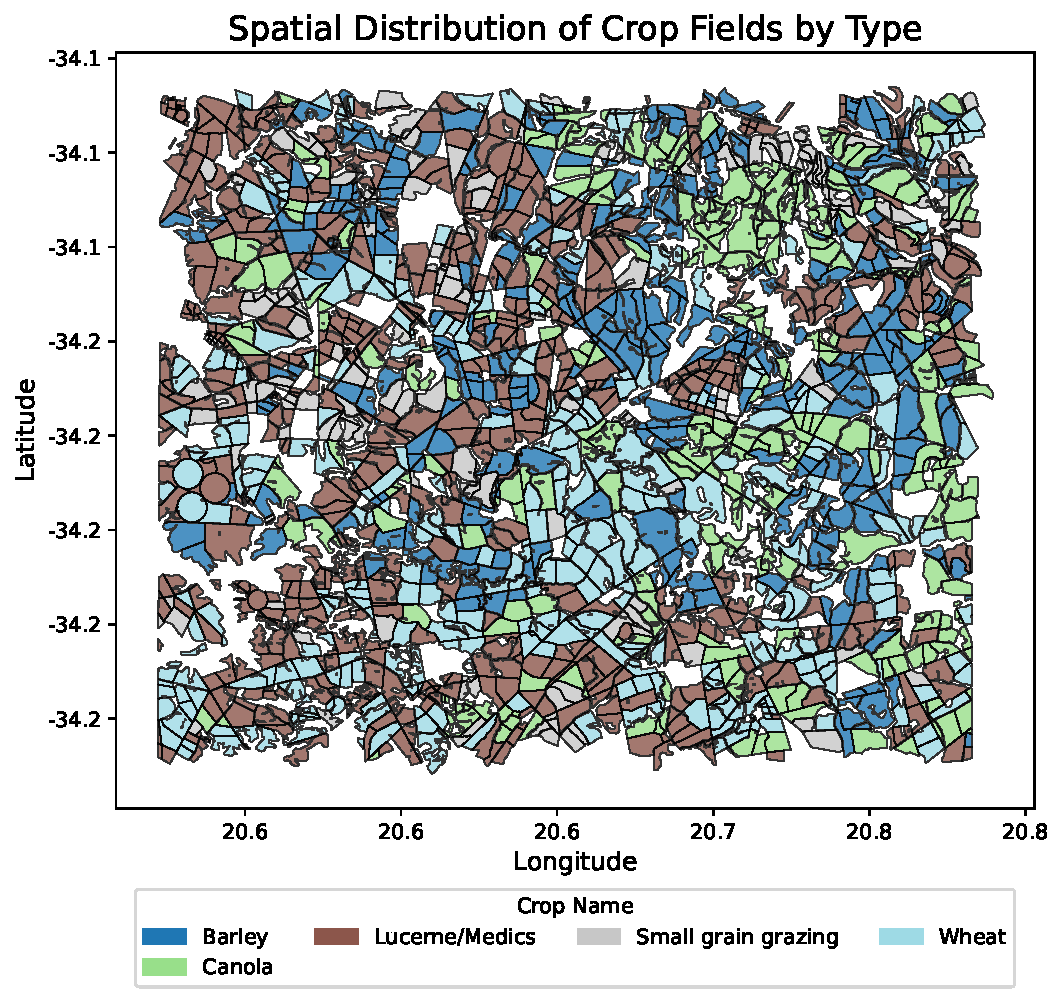
\includegraphics[width=\columnwidth]{field_boundaries_by_crop.pdf}
\caption{Field-level aggregation of pixel features: pixel values are grouped by field polygon and
summarized into a single feature vector per field.}
\label{sfig:fieldagg}
\end{figure}

\subsection{Deep Model Definitions}
\paragraph{CNN-BiLSTM} An input tensor of shape $(B,6,T)$ passes a 1D convolution (64 filters,
kernel 5) and a bidirectional LSTM (hidden size 64), with the final timestep classified via a
softmax head (Fig.~\ref{sfig:bilstm}). Class imbalance is handled with focal loss
$\mathcal{L}_{\text{focal}} = -\alpha_t (1-p_t)^{\gamma}\log(p_t)$, $\gamma=2.0$, $\alpha_t$ the
inverse class frequency. Five seeds are ensembled by averaging logits.

\begin{figure}[!t]
\centering
\includegraphics[width=\columnwidth]{cnn_bilstm.pdf}
\caption{Architecture of the CNN + BiLSTM model: 1D convolutional temporal feature extraction
followed by a bidirectional LSTM.}
\label{sfig:bilstm}
\end{figure}

\paragraph{TabNet} At each of $n_{\text{steps}}$ decision steps, an attentive transformer produces a
sparse feature mask via \emph{sparsemax},
\begin{equation}
\begin{aligned}
\mathbf{M}[i]&=\operatorname{sparsemax}\!\big(\mathbf{P}[i-1]\odot h_i(\mathbf{a}[i-1])\big),\\
\mathbf{P}[i]&=\textstyle\prod_{j=1}^{i}\big(\gamma-\mathbf{M}[j]\big),
\end{aligned}
\end{equation}
with relaxation $\gamma=1.5$; the masked features are handled by a feature transformer. We use
$n_d=n_a=64$, 5 decision steps, batch size 1024, and ensemble five seeds by averaging softmax
outputs. The sparsemax masks are the mechanism the main paper's L-TAE-S grafts onto a
temporal-attention backbone \cite{tabnet_orig, tabnet2024}.

\paragraph{L-TAE} Given an embedded sequence $\{\mathbf{z}_t\}_{t=1}^{T}$, a learned master query
attends over time; for a single head
\begin{equation}
\mathbf{o} = \sum_{t=1}^{T}\alpha_t\,\mathbf{v}_t,
\qquad
\alpha_t = \frac{\exp(\mathbf{q}^\top\mathbf{k}_t/\sqrt{d})}{\sum_{t'}\exp(\mathbf{q}^\top\mathbf{k}_{t'}/\sqrt{d})},
\end{equation}
with channel grouping keeping the encoder lightweight \cite{ltae2020}. Evaluated at pixel and field
level as a five-seed ensemble.

\paragraph{Transformer encoder} After the same band embedding and month-aware positional encoding as
L-TAE, the sequence passes three pre-norm multi-head self-attention layers
($d_{\text{model}}=128$, 8 heads, feed-forward width 256), is mean-pooled, and classified
\cite{vaswani2017, russwurm2020}. Unlike L-TAE-S it has no feature-sparsity mechanism, serving as
the capacity-versus-sparsity control. Five-seed ensemble under the same weighted-focal objective.

\paragraph{TempCNN} Stacked 1D convolutions along the temporal axis with batch normalization and
dropout, followed by a softmax head \cite{tempcnn2019}; pixel and field variants, five seeds.

\paragraph{Patch models} Each field is tiled into 100~m patches (${\sim}10\times10$ pixels) resampled
to $128\times128$ (Fig.~\ref{sfig:patches}). The multi-channel 2D CNN treats each band$\times$month
as a channel ($C=60$) through two convolutional blocks; the 3D CNN treats each patch as a
spatiotemporal volume ($T=10$, $C=6$) through three 3D-convolutional blocks with a weighted focal
loss (Fig.~\ref{sfig:patchmodel}). Both are five-seed ensembles aggregated to a field label by
majority vote.

\begin{figure}[!t]
\centering
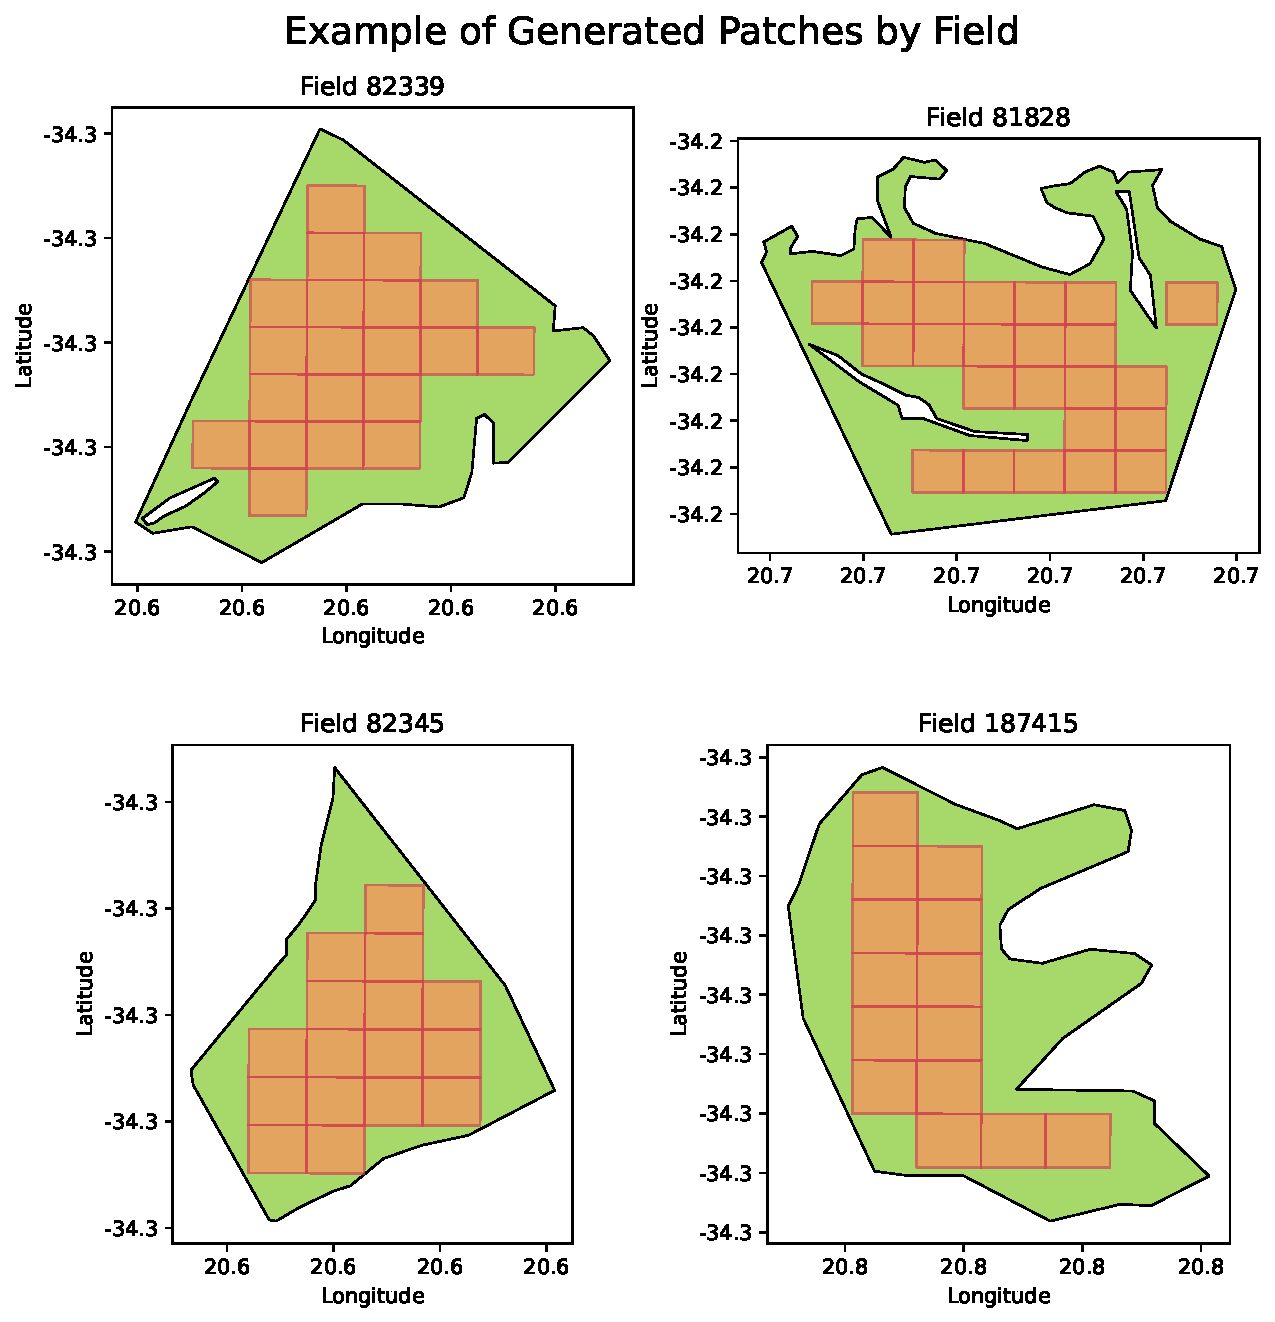
\includegraphics[width=\columnwidth]{Example_patches.pdf}
\caption{Illustration of patch generation per field.}
\label{sfig:patches}
\end{figure}

\begin{figure}[!t]
\centering
\includegraphics[width=\columnwidth]{patch_model.pdf}
\caption{Patch-level 3D CNN pipeline: each field is tiled into 100~m patches resampled to
$128\times128$; a five-seed ensemble averages softmax outputs, and per-patch predictions are
aggregated to a field label by majority vote.}
\label{sfig:patchmodel}
\end{figure}

\section{Performance Metric Definitions}
\label{sec:metrics}
\emph{Supports main paper Sec.~III.}
Let $N$ be the number of samples, $C$ the classes, and $n_c$ the support of class $c$. Cohen's Kappa
is $\kappa = (p_o - p_e)/(1 - p_e)$ with $p_o$ the observed agreement and
$p_e=\sum_c (n_{c,\text{true}}/N)(n_{c,\text{pred}}/N)$. Macro-F1 (primary) and weighted F1 are
\begin{equation}
\mathrm{F1}_{m} = \frac{1}{C}\sum_{c=1}^{C}\mathrm{F1}_c,
\quad
\mathrm{F1}_{\text{w}} = \sum_{c=1}^{C}\frac{n_c}{N}\,\mathrm{F1}_c,
\end{equation}
with $\mathrm{F1}_c = 2\,\mathrm{Prec}_c\,\mathrm{Rec}_c/(\mathrm{Prec}_c+\mathrm{Rec}_c)$.
Cross-entropy (Xent) is the AI4FoodSecurity field-level scoring metric \cite{ai4foodsecurity};
because submissions are hard labels, it is evaluated on the one-hot predicted label clipped to
$[\epsilon,1-\epsilon]$, $\epsilon=10^{-7}$:
\begin{equation}
\begin{aligned}
\mathrm{Xent} &= -\frac{1}{N}\sum_{i=1}^N \sum_{c=1}^{C} y_{i,c}\,\ln\hat{q}_{i,c},\\
\hat{q}_{i,c} &= \operatorname{clip}\!\big(\mathbb{1}[\hat{y}_i = c],\,\epsilon,\,1-\epsilon\big).
\end{aligned}
\end{equation}

\section{Training Cost}
\label{sec:cost}
\emph{Supports main paper Sec.~III and the Discussion.}
Table~\ref{stab:cost} reports wall-clock training time for a single run of each model on one
workstation (RTX 3080~Ti). The robust models that transfer best (the \texttt{xr\_fresh} tree
ensembles and the field-level L-TAE-S) are among the cheapest to train, while the most expensive
(the patch CNNs and the pixel-level Transformer) do not lead the holdout ranking.

\begin{table}[!t]
\centering
\scriptsize
\caption{Training time for a single run (one seed) of each model. Trees timed as a single
best-configuration fit, excluding the one-time Optuna search. $\dagger$Mean per seed for a 5-seed
ensemble. $\ddagger$Measured on the 75\% training fraction, the best-transferring TabNet pixel
configuration.}
\label{stab:cost}
\renewcommand{\arraystretch}{1.12}
\setlength{\tabcolsep}{6pt}
\begin{tabular}{lllr}
\toprule
\textbf{Model} & \textbf{Level} & \textbf{Features} & \textbf{Time / run} \\
\midrule
\multicolumn{4}{l}{\emph{Classical, field-level}}\\
XGBoost                & field & \texttt{xr\_fresh} & 12\,s \\
LightGBM               & field & \texttt{xr\_fresh} & 31\,s \\
Voting                 & field & \texttt{xr\_fresh} & 109\,s \\
Stacking               & field & \texttt{xr\_fresh} & 109\,s \\
SMOTE Stacked          & field & \texttt{xr\_fresh} & 99\,s \\
\midrule
\multicolumn{4}{l}{\emph{Classical, pixel-level}}\\
XGBoost                & pixel & \texttt{xr\_fresh} & 31\,s \\
LightGBM               & pixel & \texttt{xr\_fresh} & 31\,s \\
Logistic Regression    & pixel & \texttt{xr\_fresh} & 8.0\,min \\
Random Forest          & pixel & \texttt{xr\_fresh} & 73\,min \\
\midrule
\multicolumn{4}{l}{\emph{Deep, field-level (raw sequences)}}\\
TabNet (\texttt{xr\_fresh}) & field & \texttt{xr\_fresh} & 34\,s \\
TabNet (raw, field-avg) & field & raw & 39\,s \\
CNN-BiLSTM             & field & raw & 53\,s \\
L-TAE                  & field & raw & 61\,s \\
TempCNN                & field & raw & 64\,s \\
L-TAE-S                & field & raw & 18\,s\textsuperscript{$\dagger$} \\
\midrule
\multicolumn{4}{l}{\emph{Deep, pixel-level (raw sequences)}}\\
CNN-BiLSTM             & pixel & raw & 10\,min\textsuperscript{$\dagger$} \\
L-TAE-S                & pixel & raw & 24\,min\textsuperscript{$\dagger$} \\
TempCNN                & pixel & raw & 29\,min \\
L-TAE                  & pixel & raw & 38\,min \\
TabNet (raw)           & pixel & raw & 61\,min\textsuperscript{$\dagger\ddagger$} \\
Transformer            & pixel & raw & 97\,min \\
\midrule
\multicolumn{4}{l}{\emph{Deep, patch-level (raw sequences)}}\\
3D CNN                 & patch & raw & 22\,min\textsuperscript{$\dagger$} \\
Multi-Channel 2D CNN   & patch & raw & 38\,min\textsuperscript{$\dagger$} \\
\bottomrule
\end{tabular}
\end{table}

\section{Ablation Studies}
\label{sec:ablation}
\emph{Supports main paper Sec.~V (``Two Robustness Levers'').}
We attribute the holdout ranking primarily to two levers---built-in sparse feature selection and
field-level aggregation---and show that ensemble size and the imbalance-handling objective are
second-order: they shift absolute scores but never reorder the robust and fragile model groups.

\emph{(i) Field-level aggregation} (main Table~II) recovers most of the transfer gap for dense
temporal nets (L-TAE $-0.20\rightarrow-0.07$; L-TAE-S $-0.17\rightarrow-0.04$) but harms TabNet
($0.60\rightarrow0.43$). \emph{(ii) Sparse selection versus attention capacity}: a plain Transformer
with far greater capacity transfers no better than L-TAE (both ST F1$_m=0.58$), whereas grafting a
sparse channel gate (L-TAE-S) lifts transfer to $0.60$. \emph{(iii) Resampling}: the \emph{Stacking}
and \emph{SMOTE Stacked} ensembles differ only in SMOTETomek resampling; resampling widens the gap
($-0.11\rightarrow-0.21$) and lowers holdout F1$_m$ ($0.53\rightarrow0.49$).

\emph{(iv) Ensemble size} (Table~\ref{stab:ens}): seed-ensembling gives a small, monotone lift but
does not change the ordering---a single-seed L-TAE-S (F1$_m=0.56$) already exceeds the five-seed
CNN-BiLSTM and TabNet field ensembles. \emph{(v) Imbalance-handling objective}
(Table~\ref{stab:loss}): the robust L-TAE-S is almost invariant across five loss/sampler settings
($0.59$--$0.60$), whereas the fragile CNN-BiLSTM is sensitive ($0.41$--$0.56$); even CNN-BiLSTM's
best setting ($0.56$) stays below L-TAE-S's worst ($0.59$), so the objective never reorders the two.

\begin{table}[!t]
\centering
\scriptsize
\caption{Ablation (iv): spatial-transfer holdout performance versus seed-ensemble size, by
re-inference of saved per-seed checkpoints. Single-seed rows report mean$\pm$s.d.\ across five seeds.}
\label{stab:ens}
\renewcommand{\arraystretch}{1.12}
\setlength{\tabcolsep}{8pt}
\begin{tabular}{llcc}
\toprule
\textbf{Model} & \textbf{Ensemble} & \textbf{F1$_m$} & \textbf{$\kappa$} \\
\midrule
TabNet (field)     & 1 seed  & $0.31\pm0.02$ & $0.18\pm0.03$ \\
                   & 3 seeds & 0.39 & 0.29 \\
                   & 5 seeds & 0.43 & 0.34 \\
\midrule
L-TAE-S (field)    & 1 seed  & $0.56\pm0.02$ & $0.47\pm0.02$ \\
                   & 3 seeds & 0.58 & 0.50 \\
                   & 5 seeds & 0.60 & 0.52 \\
\midrule
CNN-BiLSTM (field) & 1 seed  & $0.48\pm0.02$ & $0.31\pm0.02$ \\
                   & 3 seeds & 0.52 & 0.34 \\
                   & 5 seeds & 0.51 & 0.33 \\
\bottomrule
\end{tabular}
\end{table}

\begin{table}[!t]
\centering
\scriptsize
\caption{Ablation (v): effect of the imbalance-handling objective and resampling on spatial-transfer
holdout performance (field-level, 5-seed ensembles). ``Resample'' denotes class-balanced
oversampling.}
\label{stab:loss}
\renewcommand{\arraystretch}{1.12}
\setlength{\tabcolsep}{8pt}
\begin{tabular}{lllcc}
\toprule
\textbf{Model} & \textbf{Loss} & \textbf{Resample} & \textbf{F1$_m$} & \textbf{$\kappa$} \\
\midrule
TabNet (field)     & Weighted focal ($\gamma{=}2$) & no  & 0.43 & 0.34 \\
                   & Weighted CE ($\gamma{=}0$)    & no  & 0.42 & 0.33 \\
                   & Plain CE                       & no  & 0.35 & 0.25 \\
                   & Weighted focal ($\gamma{=}2$) & yes & 0.40 & 0.23 \\
                   & Plain CE                       & yes & 0.46 & 0.37 \\
\midrule
L-TAE-S (field)    & Weighted focal ($\gamma{=}2$) & no  & 0.60 & 0.52 \\
                   & Weighted CE ($\gamma{=}0$)    & no  & 0.60 & 0.50 \\
                   & Plain CE                       & no  & 0.59 & 0.50 \\
                   & Weighted focal ($\gamma{=}2$) & yes & 0.60 & 0.49 \\
                   & Plain CE                       & yes & 0.60 & 0.50 \\
\midrule
CNN-BiLSTM (field) & Weighted focal ($\gamma{=}2$) & no  & 0.51 & 0.34 \\
                   & Weighted CE ($\gamma{=}0$)    & no  & 0.49 & 0.34 \\
                   & Plain CE                       & no  & 0.41 & 0.30 \\
                   & Weighted focal ($\gamma{=}2$) & yes & 0.56 & 0.39 \\
                   & Plain CE                       & yes & 0.50 & 0.34 \\
\bottomrule
\end{tabular}
\end{table}

\section{Data Efficiency Under Spatial Transfer}
\label{sec:efficiency}
\emph{Supports main paper contribution~5 (data efficiency), reported in Sec.~V.}
Retraining a representative set on random subsets of $75\%$, $50\%$, and $25\%$ of the training
fields and re-evaluating on the holdout (Fig.~\ref{sfig:reduction}) shows the most robust models are
also the most data-efficient: TabNet retains essentially full holdout accuracy down to a quarter of
the fields (F1$_m=0.60, 0.62, 0.62, 0.59$ at $100/75/50/25\%$), logistic regression is similarly flat
($0.56$--$0.60$), and L-TAE-S tracks them ($0.60, 0.61, 0.56, 0.58$), whereas the dense pixel L-TAE
is noisier and stays below the best transferers throughout ($0.58, 0.57, 0.53, 0.57$). Holdout
accuracy is therefore limited far more by spatial transfer than by training-set size for the robust
models.

\begin{figure}[!t]
\centering

\includegraphics[width=\columnwidth]{field_reduction.pdf}
\caption{Spatial-transfer macro-F1 versus fraction of training fields. Robust models (TabNet,
logistic regression, L-TAE-S) are nearly flat.}
\label{sfig:reduction}
\end{figure}

\section{Raw Reflectance Versus \texttt{xr\_fresh}}
\label{sec:repr}
\emph{Supports the raw-versus-\texttt{xr\_fresh} supporting experiment discussed in Sec.~V.}
Because the best-transferring classical learners in main Table~I are exactly those fed
\texttt{xr\_fresh} statistics, representation and model family are confounded there. To separate them
we trained a single XGBoost learner once on raw monthly reflectance and once on per-pixel
\texttt{xr\_fresh} statistics, holding the FID-wise splits, preprocessing, and field-level mean
pooling fixed (Table~\ref{stab:repr}). The two representations are essentially indistinguishable
under transfer (F1$_m=0.59$ raw vs.\ $0.56$ \texttt{xr\_fresh}; equal on weighted-F1 and $\kappa$;
\texttt{xr\_fresh} marginally better on cross-entropy). The \texttt{xr\_fresh} representation
therefore yields no measurable transfer-accuracy gain over raw reflectance for the trees; its value
is operational---a compact, fast-to-fit, agronomically interpretable vector
(Sec.~\ref{sec:cost})---rather than an accuracy advantage. Figure~\ref{sfig:pixfield} visualizes the
pixel-versus-field aggregation effect summarized in main Table~II.

\begin{table}[!t]
\centering
\caption{Raw reflectance versus \texttt{xr\_fresh} for a single fixed XGBoost learner, identical
splits and pooling; only the input representation differs.}
\label{stab:repr}
\renewcommand{\arraystretch}{1.1}
\setlength{\tabcolsep}{6pt}
\footnotesize
\begin{tabular}{llcccc}
\toprule
\textbf{Representation} & \textbf{Split} & \textbf{F1$_m$} & \textbf{wF1} & \textbf{$\kappa$} & \textbf{Xent} \\
\midrule
Raw reflectance    & In-region        & 0.73 & 0.80 & 0.71 & 0.65 \\
\texttt{xr\_fresh} & In-region        & 0.72 & 0.76 & 0.68 & 0.74 \\
\midrule
Raw reflectance    & Spatial transfer & 0.59 & 0.69 & 0.50 & 0.85 \\
\texttt{xr\_fresh} & Spatial transfer & 0.56 & 0.69 & 0.50 & 0.82 \\
\bottomrule
\end{tabular}
\end{table}

\begin{figure}[!t]
\centering

\includegraphics[width=\columnwidth]{pixel_vs_field.pdf}
\caption{Spatial-transfer macro-F1 at pixel versus field level. Field-level aggregation recovers
transfer for dense temporal models (L-TAE, CNN-BiLSTM) but collapses the sparsity-reliant TabNet.
Error bars are 95\% bootstrap CIs over holdout fields.}
\label{sfig:pixfield}
\end{figure}

\begin{thebibliography}{99}
\bibitem{mann2023}
Mann ML, Colson L, Nealon R, Engstrom R, Nakacwa S (2023) Lite Learning: Efficient Crop Classification in Tanzania Using Traditional Machine Learning \& Crowd Sourcing. \textit{SSRN Preprint}.
\bibitem{mann2025}
Mann ML (2025) xr\_fresh: Automated Time Series Feature Extraction for Remote Sensing and Gridded Data. \textit{J Open Source Softw} 10(115):9009. \href{https://doi.org/10.21105/joss.09009}{https://doi.org/10.21105/joss.09009}
\bibitem{james2013}
James G, Witten D, Hastie T, Tibshirani R (2013) \textit{An Introduction to Statistical Learning}. Springer.
\bibitem{breiman2001}
Breiman L (2001) Random forests. \textit{Machine Learning} 45(1):5--32. \href{https://doi.org/10.1023/A:1010933404324}{https://doi.org/10.1023/A:1010933404324}
\bibitem{ke2017}
Ke G, Meng Q, Finley T, et al. (2017) LightGBM: A highly efficient gradient boosting decision tree. \textit{NeurIPS} 30.
\bibitem{chen2016}
Chen T, Guestrin C (2016) XGBoost: A scalable tree boosting system. In: \textit{Proc 22nd ACM SIGKDD Int Conf Knowl Discov Data Min}, pp 785--794. \href{https://doi.org/10.1145/2939672.2939785}{https://doi.org/10.1145/2939672.2939785}
\bibitem{friedman2001}
Friedman JH (2001) Greedy function approximation: A gradient boosting machine. \textit{Ann Stat} 29(5):1189--1232. \href{https://doi.org/10.1214/aos/1013203451}{https://doi.org/10.1214/aos/1013203451}
\bibitem{tabnet_orig}
Arik SÖ, Pfister T (2021) TabNet: Attentive Interpretable Tabular Learning. \textit{Proc AAAI Conf Artif Intell} 35(8):6679--6687. \href{https://doi.org/10.1609/aaai.v35i8.16826}{https://doi.org/10.1609/aaai.v35i8.16826}
\bibitem{tabnet2024}
Muruganantham P, Wibowo S, Grandhi S, Islam N (2024) A Deep Learning Approach for Dealing with Tabular Data in Crop Classification. \textit{Proc IEEE Int Conf ICT Convergence (ICTC)}:2054--2059. doi:10.1109/ICTC62082.2024.10826760
\bibitem{ltae2020}
Garnot VSF, Landrieu L (2020) Lightweight Temporal Self-attention for Classifying Satellite Images Time Series. In: \textit{Advanced Analytics and Learning on Temporal Data (AALTD 2020), ECML PKDD Workshops}, LNCS vol 12588, pp 171--181. Springer. \href{https://doi.org/10.1007/978-3-030-65742-0_12}{https://doi.org/10.1007/978-3-030-65742-0\_12}
\bibitem{vaswani2017}
Vaswani A, Shazeer N, Parmar N, Uszkoreit J, Jones L, Gomez AN, Kaiser \L{}, Polosukhin I (2017) Attention Is All You Need. In: \textit{Advances in Neural Information Processing Systems (NeurIPS)}, vol 30, pp 5998--6008. \href{https://arxiv.org/abs/1706.03762}{arXiv:1706.03762}
\bibitem{russwurm2020}
Ru\ss{}wurm M, K\"orner M (2020) Self-attention for raw optical Satellite Time Series Classification. \textit{ISPRS J Photogramm Remote Sens} 169:421--435. \href{https://doi.org/10.1016/j.isprsjprs.2020.06.006}{https://doi.org/10.1016/j.isprsjprs.2020.06.006}
\bibitem{tempcnn2019}
Pelletier C, Webb GI, Petitjean F (2019) Temporal Convolutional Neural Network for the Classification of Satellite Image Time Series. \textit{Remote Sens} 11(5):523. \href{https://doi.org/10.3390/rs11050523}{https://doi.org/10.3390/rs11050523}
\bibitem{ai4foodsecurity}
AI4EO (2021) AI4FoodSecurity Challenge (South Africa), European Space Agency (ESA), in partnership with Planet, TUM, DLR and Radiant Earth. \href{https://platform.ai4eo.eu/ai4food-security-south-africa}{https://platform.ai4eo.eu/ai4food-security-south-africa}
\end{thebibliography}


\end{document}
